% !TeX root = it-governance-risk-compliance.tex
% !TeX encoding = UTF-8
\chapter{Orientasi Mata Kuliah dan Dasar-Dasar GRC}

\section*{Tujuan Pembelajaran}
\begin{itemize}
  \item Membedakan tata kelola, manajemen, risiko, kontrol, kepatuhan, dan asurans
  dengan contoh dari organisasi tempat bekerja.
  \item Menjelaskan peran mata kuliah ini dalam capstone bersama dan luaran yang
  disumbangkan ke tiap tonggak.
  \item Memetakan pemangku kepentingan dan pemicu GRC pada organisasi yang dipilih tim.
\end{itemize}

\section{Pendahuluan}

Insiden data sering memunculkan tiga jawaban yang berbeda. Unit teknologi menunjuk
konfigurasi, pengadaan menunjuk kontrak, dan vendor menunjuk instruksi pelanggan.
Ketiganya mungkin benar, tetapi organisasi masih belum menjawab siapa yang harus
memutuskan perbaikan dan siapa yang memeriksa hasilnya. Medikara Health menghadapi
keadaan ini setelah kebocoran data pasien lewat vendor pada 2025. Tata kelola diperlukan
agar keputusan, pelaksanaan, dan pertanggungjawaban saling terhubung.

Mata kuliah ini memakai istilah teknologi informasi (TI) untuk seluruh pemanfaatan
informasi dan teknologi dalam layanan organisasi. \textit{Governance, Risk, and Compliance}
(GRC) menghubungkan arah organisasi, ketidakpastian yang mengancamnya, serta kewajiban
yang harus dipenuhi. Analisis dimulai dari layanan pasien dan keputusan organisasi, bukan
dari daftar produk keamanan. Bab ini sekaligus membuka semester: tim terbentuk, organisasi
terpilih, dan profil awal masuk ke tonggak C1 capstone.

\IfFileExists{../figures/ch01-diagram-konsep.png}{%

Gambar \ref{fig:ch01-ilustrasi-bab} merangkum hubungan komponen dan konsep utama bab ini.
\begin{figure}[!htb]
  \centering
  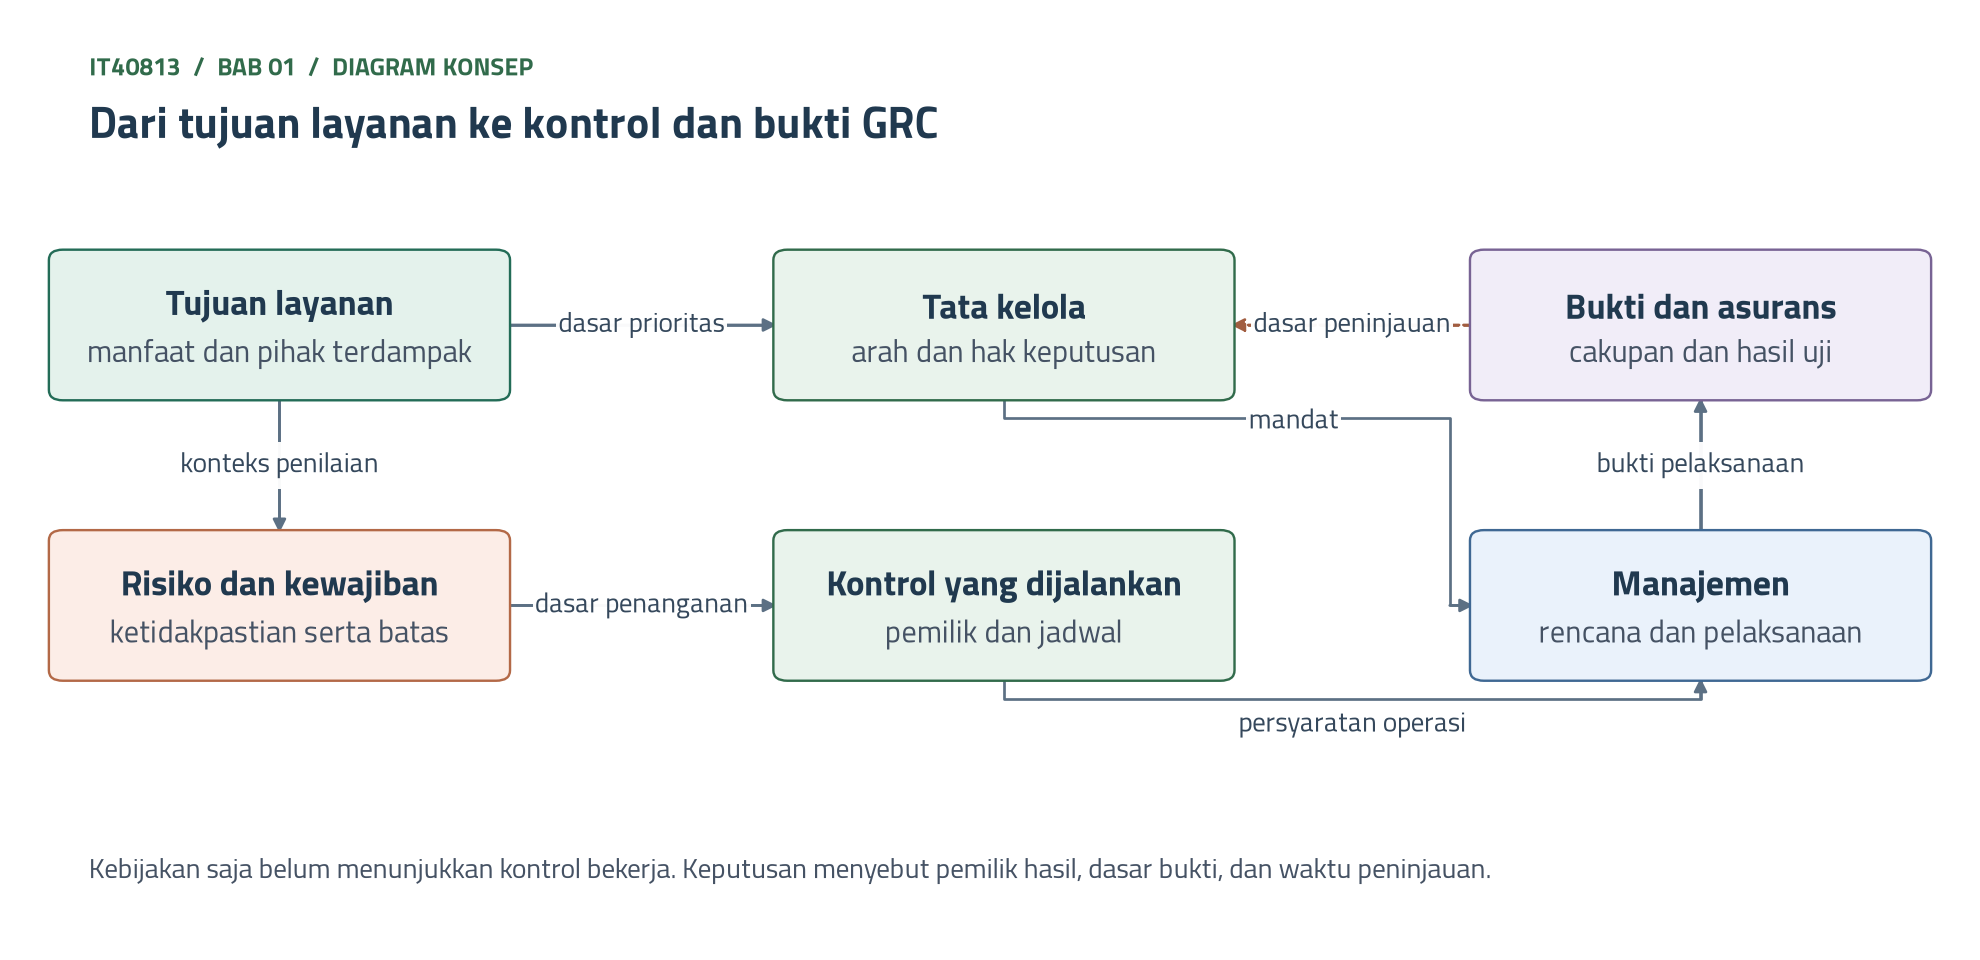
\includegraphics[width=\textwidth]{../figures/ch01-diagram-konsep.png}
  \caption{Dari tujuan layanan ke kontrol dan bukti GRC}
  \label{fig:ch01-ilustrasi-bab}
\end{figure}
}{}

Dua rujukan utama bab ini berasal dari International Organization for Standardization (ISO)
bersama International Electrotechnical Commission (IEC), serta dari ISACA. ISO/IEC
38500:2024 menjadi acuan arah dan pengawasan pemanfaatan TI. Control Objectives for
Information and Related Technologies (COBIT) 2019 membantu menghubungkan tujuan organisasi
dengan sistem tata kelola. Istilah GRC mengikuti Open Compliance and Ethics Group (OCEG)
serta Racz, Weippl, dan Seufert. Pembagian peran asurans mengikuti Three Lines Model dari
The Institute of Internal Auditors (IIA). Semua rujukan dipakai sebagai alat berpikir, lalu
diuji terhadap bukti pada kasus Medikara Health
\cite{iso38500-2024,cobit2019-intro,c01-oceg-grc,c01-racz2010,iia-tlm2026}.

\section{Mengapa Organisasi Membutuhkan Tata Kelola TI}

Tata kelola TI menetapkan arah, hak keputusan, dan cara meminta pertanggungjawaban atas
pemanfaatan TI. Weill dan Ross memandangnya sebagai penghubung antara keputusan TI dan
tujuan perusahaan, sekaligus pemantau kinerja dan akuntabilitas \cite{weill2004}. Masalah
teknis menjadi masalah tata kelola ketika pilihan tersebut memengaruhi manfaat, risiko,
sumber daya, atau hak pihak lain. Membeli aplikasi tidak menyelesaikan masalah bila
pemilik manfaat dan batas risikonya belum ditentukan.

Keputusan yang baik menyebut masalah layanan, alternatif, pihak terdampak, dasar
keputusan, serta waktu peninjauan. Satu pihak boleh mengusulkan pembelian dan pihak lain
menyetujuinya. Organisasi tetap membutuhkan pemilik hasil bisnis yang bertanggung jawab
setelah proyek selesai.

Analoginya seperti pengelola gedung. Pengelola tidak cukup membeli alarm kebakaran.
Pengelola menetapkan siapa memeriksa alarm, siapa memimpin evakuasi, dan bagaimana
penghuni mengetahui jalur keluar. Tata kelola TI memerlukan hubungan serupa antara tujuan,
pelaksana, dan pemeriksa.

Dua contoh penerapannya:
\begin{enumerate}
  \item Misalkan antrean pendaftaran pada 18 klinik turun dari 40 menjadi 25 menit
  setelah perubahan proses dan aplikasi. Direktur pelayanan menjadi pemilik hasil,
  sedangkan kepala TI bertanggung jawab pada kesiapan sistem. Bila waktu tunggu naik lagi
  dari 25 menit, direksi tahu siapa yang pertama diminta menjelaskan.
  \item Misalkan integrasi baru untuk Medikara+ menelan Rp450 juta per tahun. Dengan
  28.000 janji temu per bulan, atau 336.000 per tahun, biayanya sekitar Rp1.340 per janji
  temu. Keputusan menyetujuinya harus dibandingkan dengan nilai layanan serta biaya
  mempertahankan integrasi lama, bukan hanya harga implementasi.
\end{enumerate}

\subsection*{Tiga gejala yang memaksa organisasi bertanya}

Pertanyaan kemudian muncul: kapan kekosongan tata kelola mulai terasa? Umumnya lewat tiga
gejala, yaitu proyek gagal, data bocor, dan temuan audit.

Gejala pertama adalah proyek gagal. Flyvbjerg dan Budzier mempelajari 1.471 proyek TI.
Rata-rata pembengkakan biaya hanya 27 persen. Namun sekitar satu dari enam proyek masuk
kelompok ekstrem, dengan pembengkakan biaya rata-rata 200 persen dan keterlambatan jadwal
hampir 70 persen \cite{c01-flyvbjerg2011}. Misalkan Medikara menganggarkan Rp10 miliar untuk
modernisasi. Angka rata-rata berarti Rp12,7 miliar. Angka kelompok ekstrem berarti Rp30
miliar. Selisih sebesar itu bukan lagi urusan jadwal. Organisasi perlu tahu siapa yang
berhak menghentikan proyek dan pada batas apa.

Gejala kedua adalah data bocor. Laporan Verizon 2026 mencatat keterlibatan pihak ketiga
pada 48 persen pelanggaran data, naik dari 30 persen pada edisi sebelumnya
\cite{c01-verizon-dbir2026}. Laporan IBM 2026 mencatat rata-rata biaya pelanggaran data
global 4,99 juta dolar Amerika Serikat, dari 602 organisasi \cite{ibm-cdb2026}. Kedua angka
tidak boleh langsung dipindahkan ke Medikara, karena populasi dan cara hitungnya berbeda.
Laporan industri dipakai untuk mengajukan pertanyaan yang tepat, bukan untuk meramal
kerugian satu organisasi.

Gejala ketiga adalah temuan audit. Fakta dasar Medikara memuat temuan audit internal
tentang kontrol akses yang lemah. Misalkan audit memeriksa 30 dari 120 akun vendor dan
menemukan 6 akun masih aktif setelah penugasan berakhir, atau 20 persen sampel. Bila
sampel mewakili populasi, sekitar 24 akun bermasalah. Bila sampel dipilih tidak acak,
perkiraan itu gugur. Temuan baru bermakna ketika punya pemilik, tenggat, dan bukti
penutupan.

Tabel~\ref{tab:ch01-pemicu} merangkum empat pemicu GRC Medikara dan pertanyaan keputusan
yang menyertainya.
\begin{table}[!htb]
  \centering\small
  \caption{Pemicu GRC dan pertanyaan keputusan}\label{tab:ch01-pemicu}
  \begin{tabularx}{\textwidth}{|>{\raggedright\arraybackslash}p{0.27\textwidth}|>{\raggedright\arraybackslash}X|>{\raggedright\arraybackslash}X|}
    \hline
    \textbf{Pemicu} & \textbf{Pertanyaan organisasi} & \textbf{Bukti awal} \\ \hline
    Kebocoran vendor 2025 & Siapa membatasi akses vendor? & Kontrak dan daftar akun \\
    \hline
    Temuan kontrol akses & Siapa menutup temuan dan kapan? & Laporan audit \\ \hline
    Antrean panjang & Siapa memiliki hasil layanan? & Waktu tunggu agregat \\ \hline
    Biaya integrasi tinggi & Integrasi mana yang memberi nilai? & Biaya dan manfaat \\
    \hline
  \end{tabularx}
\end{table}

\begin{kasus}[title={Kasus Medikara Health: Insiden Vendor 2025 dalam Data Latihan}]
Fakta dasar kasus hanya menyebut kebocoran data pasien skala kecil lewat vendor pada 2025.
Mata kuliah IT40613 menambahkan data latihan berikut, dan bab ini memakai angka yang sama.
Misalkan kontrak pekerjaan vendor sudah selesai, tetapi akun dukungan vendor tetap aktif.
Selama 8 malam akun itu memanggil data kunjungan pada dua rumah sakit, 155 panggilan per
malam, sehingga 1.240 rekam kunjungan terbaca tanpa hubungan layanan dengan pekerjaan
vendor. Medikara baru mengetahuinya pada hari ke-11, lewat keluhan pasien.

Angka 1.240 setara sekitar 0,1 persen dari 1,2 juta kunjungan per tahun. Biaya langsung
latihan ini hanya Rp23,7 juta, belum termasuk sanksi, kehilangan kepercayaan, dan akibat
bagi pasien. Dua angka kecil itu tidak menjawab pertanyaan tata kelola. Siapa berwenang
mencabut akun ketika kontrak berakhir? Siapa memantau pemakaiannya? Siapa memutuskan
pemberitahuan kepada pasien? Bab 7 memakai data latihan ini dan menambahkan jamnya: hari
ke-1 Selasa pukul 20.00 WIB dan hari ke-11 Jumat pukul 20.00 WIB, lalu menghitung tenggat dari
kronologi itu.
\end{kasus}

\section{Tata Kelola dan Manajemen}

Pertanyaan berikutnya: siapa menetapkan arah, dan siapa menjalankannya? Tata kelola menilai
pilihan, memberi arah, dan memantau hasil. Manajemen menerjemahkan
arah menjadi rencana, pelaksanaan, serta pengendalian operasi. Keduanya bekerja berulang:
manajemen membawa bukti dan masalah baru, lalu pihak berwenang meninjau keputusan bila
konteks berubah.

COBIT 2019 memisahkan keduanya secara tegas. Tata kelola bekerja lewat \textit{Evaluate,
Direct, and Monitor}. Manajemen bekerja lewat \textit{Plan, Build, Run, and Monitor}, sesuai
arah dari badan pengarah. Dari 40 objektif dalam lima domain, satu domain berisi tata
kelola dan empat domain berisi manajemen \cite{cobit2019-intro}. ISO/IEC 38500:2024 memakai
tiga tugas yang sama untuk badan pengarah \cite{iso38500-2024}. Bab 2 dan Bab 4 membahas
rinciannya. Gambar~\ref{fig:ch01-tata-kelola-manajemen} memperlihatkan pembagian dan arus
informasi di antara keduanya.

\begin{figure}[!htb]
  \centering
  \begin{tikzpicture}[
  pita/.style={draw,rounded corners,fill=praditagreen!15,minimum width=11.4cm,
    minimum height=1.95cm},
  pita2/.style={pita,fill=orange!12},
  judul/.style={font=\scriptsize\bfseries,anchor=north west},
  tahap/.style={draw,rounded corners,align=center,minimum height=0.85cm,
    font=\scriptsize,fill=blue!8},
  panah/.style={-{Stealth[length=2mm]},thick}
]
  \node[pita] (atas) at (5.7,3.55) {};
  \node[judul] at (atas.north west) {Tata kelola: badan pengarah};
  \node[tahap,text width=3cm] at (1.8,3.3)
    {\textit{Evaluate}\\{\tiny\mdseries menilai pilihan dan akibat}};
  \node[tahap,text width=3cm] at (5.7,3.3)
    {\textit{Direct}\\{\tiny\mdseries memberi arah dan batas}};
  \node[tahap,text width=3cm] at (9.6,3.3)
    {\textit{Monitor}\\{\tiny\mdseries memantau hasil dan kepatuhan}};

  \node[pita2] (bawah) at (5.7,0) {};
  \node[judul] at (bawah.north west) {Manajemen: pelaksana sesuai mandat};
  \node[tahap,text width=2.2cm] at (1.35,-0.25)
    {\textit{Plan}\\{\tiny\mdseries merencanakan}};
  \node[tahap,text width=2.2cm] at (4.25,-0.25)
    {\textit{Build}\\{\tiny\mdseries membangun}};
  \node[tahap,text width=2.2cm] at (7.15,-0.25)
    {\textit{Run}\\{\tiny\mdseries menjalankan}};
  \node[tahap,text width=2.2cm] at (10.05,-0.25)
    {\textit{Monitor}\\{\tiny\mdseries memantau operasi}};

  \draw[panah] (3.1,2.56) -- node[left,font=\scriptsize,align=right]
    {mandat, prioritas,\\dan batas} (3.1,1);
  \draw[panah] (8.3,1) -- node[right,font=\scriptsize,align=left]
    {bukti pelaksanaan\\dan masalah baru} (8.3,2.56);
\end{tikzpicture}

  \caption{Pembagian tugas dan arus informasi antara tata kelola dan manajemen}
  \label{fig:ch01-tata-kelola-manajemen}
\end{figure}

Analoginya seperti pemilik restoran dan manajer dapur. Pemilik menentukan jenis layanan,
batas harga, dan standar kebersihan. Manajer dapur menyusun giliran kerja dan memeriksa
bahan setiap pagi. Pemilik tetap meminta laporan mutu, tetapi tidak perlu memilih urutan
memasak setiap pesanan.

Dua contoh penerapannya:
\begin{enumerate}
  \item Misalkan direksi menyetujui modernisasi lima rumah sakit dengan syarat layanan
  tetap berjalan. Manajemen menyusun jadwal migrasi bertahap dan prosedur pemulihan.
  Syarat itu keputusan tata kelola. Urutan kelima rumah sakit adalah keputusan manajemen.
  \item Misalkan komite hanya menerima laporan 90 persen pekerjaan selesai. Tanpa
  menilai manfaat dan risiko yang tersisa, komite belum memiliki dasar untuk mengizinkan
  peluncuran. Sisa 10 persen bisa saja berisi pekerjaan yang paling menentukan.
\end{enumerate}

Tabel~\ref{tab:ch01-peran} merangkum pembagian arah dan pelaksanaan pada tiga keputusan
Medikara.
\begin{table}[!htb]
  \centering\small
  \caption{Pembagian arah dan pelaksanaan}\label{tab:ch01-peran}
  \begin{tabularx}{\textwidth}{|>{\raggedright\arraybackslash}p{0.27\textwidth}|>{\raggedright\arraybackslash}X|>{\raggedright\arraybackslash}X|}
    \hline
    \textbf{Keputusan} & \textbf{Tata kelola} & \textbf{Manajemen} \\ \hline
    Identitas pasien tunggal & Tetapkan tujuan dan pemilik manfaat & Susun rencana
    integrasi \\ \hline
    Akses vendor & Tetapkan batas dan penanggung jawab & Berikan dan cabut akun \\
    \hline
    Investasi layanan & Pilih prioritas dan batas biaya & Kelola kontrak dan jadwal \\
    \hline
  \end{tabularx}
\end{table}

\subsection*{Jabatan bukan penentu}

Dua hal sering tertukar: jabatan penanda tangan dan jenis keputusan. Pembagiannya begini.
Memberi persetujuan atas batas investasi berbeda dari menyetujui jadwal pemasangan server.
Keputusan pertama mengalokasikan sumber daya dan menerima konsekuensi organisasi. Keputusan
kedua menjalankan rencana dalam kewenangan yang sudah diberikan. Seorang direktur yang
menandatangani jadwal sedang menjalankan manajemen. Seorang kepala TI yang ikut memilih
prioritas investasi di komite sedang ikut dalam tata kelola.

Pembedaan ini punya dua konsekuensi. Pertama, batas eskalasi harus tertulis. Misalkan
direksi menyetujui integrasi Rp450 juta per tahun dengan toleransi 10 persen, sehingga batas
atasnya Rp495 juta. Kenaikan menjadi Rp480 juta masih dalam kewenangan manajemen. Kenaikan
menjadi Rp540 juta, atau 20 persen, kembali ke direksi. Kedua, isi laporan ke direksi
berubah. Laporan tidak perlu memuat jadwal pemasangan di 18 klinik satu per satu. Laporan
memuat manfaat, risiko sisa, dan pilihan yang menunggu keputusan.

\section{Istilah Dasar GRC}

Keputusan dan pelaksanaan memerlukan bahasa yang sama. Apa beda risiko, kontrol, kepatuhan,
dan asurans? ISO 31000:2018 mendefinisikan risiko sebagai efek ketidakpastian terhadap tujuan, dan
kontrol sebagai tindakan yang mempertahankan atau mengubah risiko \cite{iso31000-2018}.
Kepatuhan adalah pemenuhan kewajiban yang berlaku, baik dari hukum, kontrak, maupun
komitmen yang dipilih organisasi. Asurans, menurut IIA, adalah pernyataan yang dimaksudkan
untuk meningkatkan keyakinan pemangku kepentingan atas proses tata kelola, manajemen
risiko, kepatuhan, dan kontrol \cite{iia-tlm2026}. Keyakinan itu lahir dari penilaian
berbasis bukti. Keempat istilah terhubung, tetapi menjawab pertanyaan berbeda.

Analoginya seperti aturan kas kecil. Aturan menetapkan batas pengeluaran, bukti kuitansi,
dan pihak yang menyetujui. Kuitansi menunjukkan transaksi terjadi. Pemeriksaan silang
terhadap buku kas memberi keyakinan bahwa aturan benar-benar dijalankan.

Dua contoh penerapannya:
\begin{enumerate}
  \item Misalkan risiko R-01 adalah akses vendor yang berlebihan menyebabkan
  pengungkapan data pasien. Kontrol AC-01 berupa peninjauan akses berkala menguji apakah
  hak akses masih diperlukan. Kode R-01 dan AC-01 tetap dipakai sampai Bab 14.
  \item Misalkan seluruh karyawan yang berjumlah sekitar 4.800 orang sudah menandatangani
  kebijakan akses, tetapi 6 dari 30 akun vendor yang diperiksa belum dicabut setelah
  penugasan berakhir. Kepatuhan administratif belum membuktikan efektivitas pencabutan
  akses.
\end{enumerate}

Tabel~\ref{tab:ch01-istilah} merangkum istilah GRC dan bukti penerapannya.
\begin{table}[!htb]
  \centering\small
  \caption{Istilah GRC dan bukti penerapannya}\label{tab:ch01-istilah}
  \begin{tabularx}{\textwidth}{|>{\raggedright\arraybackslash}p{0.22\textwidth}|>{\raggedright\arraybackslash}X|>{\raggedright\arraybackslash}X|}
    \hline
    \textbf{Istilah} & \textbf{Pertanyaan} & \textbf{Contoh bukti} \\ \hline
    Tata kelola & Siapa memutuskan arah dan batas? & Notulen dan delegasi \\ \hline
    Manajemen & Bagaimana arah dijalankan? & Rencana dan laporan kerja \\ \hline
    Risiko & Apa yang mengancam tujuan? & Skenario R-01 \\ \hline
    Kontrol & Apa yang mengubah risiko? & Hasil peninjauan AC-01 \\ \hline
    Kepatuhan & Kewajiban mana yang dipenuhi? & Register kewajiban \\ \hline
    Asurans & Mengapa hasil layak dipercaya? & Kertas kerja pengujian \\ \hline
  \end{tabularx}
\end{table}

\begin{kasus}[title={Kasus Medikara Health: Dari Insiden ke Pemilik Keputusan}]
Kebocoran data skala kecil melalui vendor pada 2025 adalah fakta kasus. Misalkan tim
menelusuri insiden itu ke akun dukungan yang masih aktif setelah kontrak pekerjaan
selesai. Tim mencatat R-01, menetapkan pemilik risiko pada fungsi bisnis yang menentukan
pemrosesan, dan mengusulkan AC-01. Bukti yang diminta adalah daftar akun, dasar
pemberian akses, hasil peninjauan, serta tindakan pencabutan. Besar kecilnya insiden
tidak menghilangkan kebutuhan menilai kewajiban hukum. Pasal 46 Undang-Undang (UU) Nomor
27 Tahun 2022 tentang Pelindungan Data Pribadi (PDP) mengatur pemberitahuan tertulis paling
lambat $3 \times 24$ jam \cite{uu27-2022-pdp}. Bab 7 mengujinya dengan kronologi.
\end{kasus}

\subsection*{Kebijakan, standar, prosedur, dan pedoman}

Empat dokumen ini sering tertukar. Pembagiannya begini. Kebijakan menyatakan arah dan
batas. Standar organisasi menetapkan persyaratan minimum. Prosedur menjelaskan urutan
kerja. Pedoman membantu memilih cara yang sesuai, tanpa mengikat. Kata ``standar'' di sini
berarti aturan internal organisasi, berbeda dari standar internasional seperti ISO/IEC
27001. Tabel~\ref{tab:ch01-dokumen} memakai kontrol AC-01 sebagai contoh.

\begin{table}[!htb]
  \centering\small
  \caption{Dokumen dan catatan untuk kontrol AC-01 (angka pengandaian)}
  \label{tab:ch01-dokumen}
  \begin{tabularx}{\textwidth}{|>{\raggedright\arraybackslash}p{0.22\textwidth}|>{\raggedright\arraybackslash}X|}
    \hline
    \textbf{Jenis} & \textbf{Isi pada AC-01} \\ \hline
    Kebijakan & Akses vendor hanya berlaku selama penugasan \\ \hline
    Standar organisasi & Akun dicabut paling lambat 1 hari kerja setelah penugasan berakhir,
    dan ditinjau setiap bulan \\ \hline
    Prosedur & Pengelola vendor menarik daftar akun, pemilik layanan menandai akun yang
    masih perlu, admin mencabut sisanya \\ \hline
    Pedoman & Pakai akun per orang, bukan akun bersama, bila sistem memungkinkan \\ \hline
    Catatan sebagai bukti & Peninjauan bulan berikutnya: 120 akun ditinjau, 24 akun dicabut,
    tanggal dan penanggung jawab tercatat \\ \hline
  \end{tabularx}
\end{table}

Kebijakan tanpa prosedur dan bukti pelaksanaan belum menunjukkan bahwa kontrol bekerja.
Baris terakhir pada tabel itulah yang dibaca auditor.

\subsection*{Siapa memberi keyakinan?}

Pertanyaan kemudian muncul: siapa yang memeriksa, kalau pelaksana tidak boleh menilai
pekerjaannya sendiri? Three Lines Model dari IIA membedakan peran, bukan departemen.
Manajemen sebagai lini pertama memiliki dan mengelola risiko. Peran lini kedua memberi
keahlian, dukungan, pemantauan, dan tantangan. Audit internal sebagai lini ketiga memberi
asurans yang independen dan objektif. Badan pengarah memberi arah strategis dan pengawasan
\cite{iia-tlm2026}. Tabel~\ref{tab:ch01-tiga-lini} menerapkannya pada AC-01, dengan contoh
pemilik Sistem Informasi Manajemen Rumah Sakit (SIMRS). Bab 12 membahas model ini lebih dalam.

\begin{table}[!htb]
  \centering\small
  \caption{Three Lines Model pada kontrol AC-01}\label{tab:ch01-tiga-lini}
  \begin{tabularx}{\textwidth}{|>{\raggedright\arraybackslash}p{0.22\textwidth}|>{\raggedright\arraybackslash}X|>{\raggedright\arraybackslash}X|}
    \hline
    \textbf{Peran} & \textbf{Contoh pemilik} & \textbf{Tanggung jawab} \\ \hline
    Badan pengarah & Direksi dan dewan komisaris sesuai kewenangan & Menetapkan arah dan
    meminta laporan \\ \hline
    Lini pertama & Pemilik SIMRS dan layanan & Menjalankan kontrol AC-01 \\ \hline
    Lini kedua & Risiko, privasi, keamanan & Memantau dan menantang \\ \hline
    Lini ketiga & Audit internal & Menguji secara independen \\ \hline
  \end{tabularx}
\end{table}

Pembedaan ini berlaku juga untuk vendor. IIA menegaskan bahwa kegiatan yang dialihkan ke
penyedia luar tidak berubah perannya dalam model, dan akuntabilitas badan pengarah atas
kegiatan itu tidak berubah \cite{iia-tlm2026}. Medikara dapat menyerahkan pekerjaan kepada
vendor, tetapi tidak dapat menyerahkan pertanggungjawaban atas keputusannya.

\section{GRC sebagai Satu Kesatuan}

Bila tiap istilah menjawab pertanyaan berbeda, mengapa ketiganya disatukan dalam satu
singkatan? OCEG mendefinisikan GRC sebagai kumpulan kemampuan terpadu yang memungkinkan organisasi
mencapai tujuan secara andal, sekaligus menangani ketidakpastian dan bertindak dengan
integritas \cite{c01-oceg-grc}. Racz, Weippl, dan Seufert merumuskan GRC sebagai pendekatan
terpadu dan menyeluruh terhadap tata kelola, risiko, dan kepatuhan di seluruh organisasi.
Pendekatan itu memastikan organisasi bertindak etis dan sesuai dengan \textit{risk
appetite}, kebijakan internal, serta regulasi, lewat penyelarasan strategi, proses,
teknologi, dan orang \cite{c01-racz2010,c01-racz2011}. Kedua definisi menyimpulkan hal yang
sama: GRC bukan tiga unit yang terpisah, dan bukan satu produk perangkat lunak.

Analoginya seperti pasien yang berobat ke tiga dokter tanpa rekam medis bersama. Tiap
dokter meminta pemeriksaan darah sendiri, memberi resep sendiri, dan tidak tahu obat dari
dokter lain. Setiap dokter bekerja benar menurut catatannya, tetapi pasien menanggung
biaya berlipat dan risiko obat yang saling berbenturan.

Dua contoh penerapannya:
\begin{enumerate}
  \item Misalkan audit internal, bagian kepatuhan, dan keamanan informasi masing-masing
  meminta daftar akun kepada 5 rumah sakit dan 18 klinik setiap triwulan. Jumlahnya $3
  \times 23 \times 4 = 276$ permintaan per tahun untuk bukti yang sama. Dengan satu
  register dan satu jadwal, permintaan turun menjadi $23 \times 4 = 92$. Bila satu
  permintaan memakan 2 jam kerja, fasilitas menghemat $184 \times 2 = 368$ jam per tahun.
  \item Misalkan kontrol AC-01 mendukung tiga acuan sekaligus: UU 27/2022 Pasal 35, 36, 37, dan
  39, dengan Pasal 39 sebagai acuan utama, ISO/IEC 27001:2022 Annex A 5.18, dan National
  Institute of Standards and Technology
  Cybersecurity Framework (NIST CSF) 2.0 PR.AA-05. Tanpa register bersama, satu kontrol
  tercatat tiga kali dengan tiga nama. Pemetaan ini menunjukkan kontribusi, bukan
  kesetaraan, sehingga tiap acuan tetap diperiksa pada Bab 14.
\end{enumerate}

Gambar~\ref{fig:ch01-grc-terpadu} memperlihatkan bentuk kerja terpadu. Ketiga fungsi berangkat
dari tujuan layanan yang sama dan mencatat hasilnya pada satu register.
Tabel~\ref{tab:ch01-terpadu} membandingkannya dengan cara kerja terpisah.

\begin{figure}[!htb]
  \centering
  \begin{tikzpicture}[
  kotak/.style={draw,rounded corners,align=center,minimum height=1cm,
    font=\scriptsize,fill=blue!8},
  panah/.style={-{Stealth[length=2mm]},thick}
]
  \node[kotak,fill=praditagreen!15,text width=10.4cm,minimum height=0.8cm] (tujuan)
    at (5.4,4.5) {\textbf{Tujuan layanan}: manfaat dan pihak terdampak};

  \node[kotak,text width=3cm] (g) at (1.8,2.85)
    {\textbf{Tata kelola}\\{\tiny\mdseries arah dan hak keputusan}};
  \node[kotak,text width=3cm] (r) at (5.4,2.85)
    {\textbf{Risiko}\\{\tiny\mdseries ketidakpastian serta batas}};
  \node[kotak,text width=3cm] (c) at (9,2.85)
    {\textbf{Kepatuhan}\\{\tiny\mdseries kewajiban yang berlaku}};

  \node[kotak,fill=orange!12,text width=10.4cm] (reg) at (5.4,1.2)
    {\textbf{Satu register bersama}\\
     {\tiny\mdseries ID tetap: pemicu P-01, risiko R-01, kontrol AC-01, kewajiban,
     bukti, dan pemilik}};

  \node[kotak,fill=green!10,text width=10.4cm,minimum height=0.8cm] (bukti) at (5.4,-0.4)
    {\textbf{Bukti dan asurans}: cakupan dan hasil uji};

  \draw[panah] (g.north |- tujuan.south) -- (g.north);
  \draw[panah] (r.north |- tujuan.south) -- (r.north);
  \draw[panah] (c.north |- tujuan.south) -- (c.north);
  \draw[panah] (g.south) -- (g.south |- reg.north);
  \draw[panah] (r.south) -- (r.south |- reg.north);
  \draw[panah] (c.south) -- (c.south |- reg.north);
  \draw[panah] (reg) -- (bukti);
  \draw[panah,dashed] (bukti.east) -- ++(0.45,0) |- (tujuan.east);
  \node[font=\tiny,rotate=90,fill=white,inner sep=1pt] at (11.05,2.05)
    {dasar peninjauan};
\end{tikzpicture}

  \caption{GRC terpadu: tiga fungsi berbagi satu tujuan, satu register, dan satu dasar peninjauan}
  \label{fig:ch01-grc-terpadu}
\end{figure}

\begin{table}[!htb]
  \centering\small
  \caption{Cara kerja terpisah dan terpadu}\label{tab:ch01-terpadu}
  \begin{tabularx}{\textwidth}{|>{\raggedright\arraybackslash}p{0.22\textwidth}|>{\raggedright\arraybackslash}X|>{\raggedright\arraybackslash}X|}
    \hline
    \textbf{Aspek} & \textbf{Terpisah} & \textbf{Terpadu} \\ \hline
    Pengenal & Tiap unit punya nama sendiri & ID tetap: R-01, AC-01 \\ \hline
    Permintaan bukti & 276 permintaan per tahun & 92 permintaan per tahun \\ \hline
    Laporan ke direksi & Tiga laporan, tiga skala & Satu gambaran, sumber dapat ditelusuri \\
    \hline
    Peninjauan & Menurut jadwal tiap unit & Menurut tujuan layanan dan pemicu \\ \hline
  \end{tabularx}
\end{table}

Alur yang sama tampak pada Gambar~\ref{fig:ch01-ilustrasi-bab}. Tujuan layanan memberi dasar
prioritas bagi tata kelola, dan konteks penilaian bagi risiko dan kewajiban. Tata kelola
memberi mandat kepada manajemen. Risiko dan kewajiban menjadi dasar penanganan, yang
diwujudkan dalam kontrol yang dijalankan. Kontrol menjadi persyaratan operasi bagi
manajemen. Manajemen menghasilkan bukti pelaksanaan, yang dinilai dalam bukti dan asurans.
Hasilnya menjadi dasar peninjauan bagi tata kelola, dan siklus berulang.

\subsection*{Terpadu tidak berarti dilebur}

Dua hal pada GRC sering tertukar: terpadu dan dilebur. Pembagiannya begini. Terpadu berarti
memakai tujuan, pengenal, dan bukti yang sama. Dilebur berarti satu unit mengerjakan semua
peran. Peleburan justru merusak asurans, karena pelaksana menilai pekerjaannya sendiri. IIA
menempatkan independensi sebagai dasar asurans yang dapat dipercaya, sekaligus mengingatkan
bahwa independensi tidak boleh ditafsirkan sebagai isolasi \cite{iia-tlm2026}.

Keputusan memakai satu register punya dua konsekuensi. Pertama, register memerlukan pemilik
dan aturan perubahan, karena satu kesalahan kini terbaca oleh semua unit. Kedua, organisasi
menanggung biaya menyamakan istilah di awal. Misalkan menyamakan 40 baris risiko memakan
20 jam kerja. Biaya itu sebanding bila menghemat 368 jam per tahun seperti pada contoh di
atas, tetapi belum tentu sebanding bagi organisasi yang hanya punya satu lokasi. Bab 14
membahas alat GRC, setelah cara kerjanya jelas.

\section{Peta Kerangka dan Regulasi}

Rujukan mana yang dipakai untuk pertanyaan tertentu? Kerangka menyediakan cara
mengelompokkan masalah. Standar menyediakan prinsip, panduan,
atau persyaratan sesuai jenisnya. Regulasi menetapkan kewajiban hukum dalam ruang lingkup
tertentu. Organisasi memilih kerangka berdasarkan pertanyaan yang perlu dijawab, lalu
menelusuri kewajiban ke sumber hukum aslinya.

Analoginya seperti peta jalan, aturan lalu lintas, dan buku servis kendaraan. Peta membantu
memilih rute. Aturan mengikat pengguna jalan. Buku servis membantu merawat kendaraan.
Ketiganya dapat dipakai dalam satu perjalanan tanpa saling menggantikan.

Dua contoh penerapannya:
\begin{enumerate}
  \item Misalkan Medikara perlu menetapkan siapa menerima risiko layanan. ISO/IEC 38500
  dan COBIT membantu merancang hak keputusan. Daftar konfigurasi server tidak menjawab
  pertanyaan tersebut. Medikara juga tidak perlu menjalankan semuanya sekaligus: bila 52
  staf TI menanggung 40 objektif COBIT, satu objektif hanya kebagian 1,3 orang. Karena itu
  Bab 4 memilih objektif prioritas.
  \item Misalkan tim perlu menentukan masa simpan rekam medis. Tim membaca peraturan
  sektor kesehatan terlebih dahulu, lalu mencari kontrol dan arsitektur yang
  mendukungnya. Urutan terbalik membuat 5 rumah sakit membangun fitur untuk kewajiban yang
  belum dibaca.
\end{enumerate}

Tabel~\ref{tab:ch01-kerangka} merupakan peta belajar, bukan daftar yang harus diterapkan
seluruhnya. Nama standar dicantumkan bersama versinya agar keputusan dapat ditelusuri ketika
rujukan berubah. Tabel itu memakai beberapa singkatan: Information Technology Infrastructure
Library (ITIL), Peraturan Menteri Kesehatan (Permenkes), Peraturan Pemerintah (PP), Committee
of Sponsoring Organizations of the Treadway Commission (COSO), \textit{Enterprise Risk
Management} (ERM), dan \textit{Artificial Intelligence} (AI).

\begin{table}[!htb]
  \centering\small
  \caption{Peta pertanyaan dan rujukan semester}\label{tab:ch01-kerangka}
  \begin{tabularx}{\textwidth}{|>{\raggedright\arraybackslash}p{0.27\textwidth}|>{\raggedright\arraybackslash}X|>{\raggedright\arraybackslash}p{0.17\textwidth}|>{\raggedright\arraybackslash}p{0.08\textwidth}|}
    \hline
    \textbf{Pertanyaan} & \textbf{Rujukan} & \textbf{Jenis} & \textbf{Bab} \\ \hline
    Siapa memberi arah dan memutuskan? & ISO/IEC 38500:2024 \cite{iso38500-2024} & Prinsip &
    2, 8 \\ \hline
    Bagaimana sistem tata kelola disusun? & COBIT 2019 \cite{cobit2019-intro}, ITIL
    \cite{itil4} & Kerangka & 4, 8 \\ \hline
    Aturan mana yang mengikat? & UU 27/2022 \cite{uu27-2022-pdp}, Permenkes 24/2022
    \cite{permenkes24-2022}, PP 71/2019 \cite{pp71-2019-pste} & Hukum & 3, 7 \\ \hline
    Ketidakpastian mana yang mengancam tujuan? & ISO 31000:2018 \cite{iso31000-2018}, COSO ERM
    2017 \cite{cosoerm2017} & Panduan & 5 \\ \hline
    Apakah informasi dan vendor aman? & ISO/IEC 27001:2022 \cite{iso27001-2022}, NIST CSF 2.0
    \cite{nistcsf2} & Persyaratan, kerangka & 6, 9 \\ \hline
    Apakah layanan bertahan saat gangguan? & ISO 22301:2019 \cite{iso22301-2019} & Persyaratan
    & 10 \\ \hline
    Bagaimana AI dikendalikan? & ISO/IEC 42001:2023 \cite{iso42001-2023} & Persyaratan & 11
    \\ \hline
    Mengapa hasil layak dipercaya? & Global Internal Audit Standards \cite{iia-gias2024},
    Three Lines Model \cite{iia-tlm2026} & Standar profesi, model peran & 12, 13, 14 \\ \hline
  \end{tabularx}
\end{table}

\subsection*{Patuh dan bersertifikat}

Dua hal sering tertukar: mematuhi hukum dan memegang sertifikat. Pembagiannya begini.
Regulasi berlaku karena organisasi masuk ruang lingkupnya, tanpa perlu memilih. Standar
seperti ISO/IEC 27001 dipilih organisasi, atau diminta oleh mitra lewat kontrak. Sertifikat
menunjukkan sistem manajemen memenuhi persyaratan untuk ruang lingkup tertentu. Sertifikat
tidak membuktikan pemenuhan seluruh kewajiban UU PDP. Sebaliknya, memenuhi satu pasal hukum
juga belum berarti risikonya terkendali, dan Latihan 2 menguji hal ini.

Versi rujukan perlu diperiksa ulang. Per 30 Oktober 2026, informasi produk ISACA telah
menyebut COBIT 7, sementara halaman kerangka resminya masih menyediakan publikasi COBIT
2019. PeopleCert menerbitkan ITIL (Version 5) pada 2026. ISO 31000 dan ISO 22301 sedang
direvisi. Modul ini memakai versi yang tertulis pada tabel. Tim mencatat versi yang dipakai
dan tanggal pemeriksaannya, bukan menebak isi versi berikutnya.

\section{Capstone Bersama dan Kasus Medikara Health}

Di mana semua konsep itu diterapkan? Capstone menghasilkan satu Cetak Biru Transformasi
Digital yang dipelihara bersama empat
mata kuliah. IT40513 menyusun arsitektur \textit{enterprise}, IT40613 menyusun platform dan
\textit{Application Programming Interface} (API), IT40713 merancang layanan serta
infrastruktur \textit{cloud}, dan IT40813 menetapkan tata kelola, risiko, serta kepatuhan.
Artefak harus menggunakan nama layanan, sistem, data, dan angka biaya yang sama.
Gambar~\ref{fig:ch01-capstone} memperlihatkan hubungan keempat mata kuliah dengan tonggak C1
sampai C4.

\begin{figure}[!htb]
  \centering
  \begin{tikzpicture}[
  matkul/.style={draw,rounded corners,align=center,text width=2.5cm,
    minimum height=1.25cm,font=\scriptsize,fill=blue!8},
  tonggak/.style={draw,rounded corners,align=center,text width=2.5cm,
    minimum height=1.25cm,font=\scriptsize,fill=praditagreen!15},
  panah/.style={-{Stealth[length=2mm]},thick}
]
  \node[matkul] (ea) at (0,3.3)
    {IT40513\\{\tiny\mdseries arsitektur \textit{enterprise}}};
  \node[matkul] (api) at (3.1,3.3)
    {IT40613\\{\tiny\mdseries platform dan API}};
  \node[matkul] (cloud) at (6.2,3.3)
    {IT40713\\{\tiny\mdseries layanan dan \textit{cloud}}};
  \node[matkul,fill=orange!12] (grc) at (9.3,3.3)
    {IT40813\\{\tiny\mdseries tata kelola, risiko,}\\{\tiny\mdseries dan kepatuhan}};

  \node[draw,rounded corners,align=center,fill=green!10,text width=11.4cm,
    minimum height=0.95cm,font=\scriptsize] (cetak) at (4.65,1.55)
    {\textbf{Cetak Biru Transformasi Digital}\\
     {\tiny\mdseries satu organisasi; nama layanan, sistem, data, dan biaya yang sama}};

  \foreach \sumber in {ea,api,cloud,grc}
    \draw[panah] (\sumber.south) -- (\sumber.south |- cetak.north);

  \node[tonggak] (c1) at (0,0)
    {\textbf{C1} Konteks dan Strategi\\{\tiny\mdseries Pertemuan 1 sampai 3}};
  \node[tonggak] (c2) at (3.1,0)
    {\textbf{C2} Kondisi Saat Ini\\{\tiny\mdseries Pertemuan 4 sampai 7}};
  \node[tonggak] (c3) at (6.2,0)
    {\textbf{C3} Kondisi Target\\{\tiny\mdseries Pertemuan 8 sampai 11}};
  \node[tonggak] (c4) at (9.3,0)
    {\textbf{C4} Peta Jalan dan Tata Kelola\\{\tiny\mdseries Pertemuan 12 sampai 14}};

  \draw[panah] (c1) -- (c2);
  \draw[panah] (c2) -- (c3);
  \draw[panah] (c3) -- (c4);
  \foreach \tonggak in {c1,c2,c3,c4}
    \draw[panah] (\tonggak.north |- cetak.south) -- (\tonggak.north);
\end{tikzpicture}

  \caption{Empat mata kuliah mengisi satu cetak biru lewat empat tonggak}
  \label{fig:ch01-capstone}
\end{figure}

Analoginya seperti satu rancangan gedung. Gedung memerlukan gambar arsitektur, struktur,
listrik, dan jalur evakuasi yang memakai ukuran sama. Empat gambar yang bagus tetapi berbeda
letak pintunya tidak membentuk rancangan yang dapat dibangun.

Dua contoh penerapannya:
\begin{enumerate}
  \item Misalkan IT40613 membuka API hasil laboratorium dari 1 laboratorium rujukan ke 18
  klinik. GRC harus menilai penerima data, tujuan akses, dan kontrolnya sebelum arsitektur
  target disepakati.
  \item Misalkan IT40713 memindahkan Medikara+, dengan 28.000 janji temu per bulan, ke
  \textit{cloud}. GRC meninjau tanggung jawab vendor dan persyaratan lokasi data, lalu
  mengembalikan batasan kepada tim arsitektur.
\end{enumerate}

Tabel~\ref{tab:ch01-capstone} merangkum tonggak dan kontribusi GRC. Perubahan pada satu
tonggak bisa kembali ke tonggak sebelumnya. Bila arsitektur berubah pada C3, daftar risiko
dari C2 ikut ditinjau.

\begin{table}[!htb]
  \centering\small
  \caption{Tonggak dan kontribusi GRC}\label{tab:ch01-capstone}
  \begin{tabularx}{\textwidth}{|>{\raggedright\arraybackslash}p{0.3\textwidth}|>{\raggedright\arraybackslash}p{0.16\textwidth}|>{\raggedright\arraybackslash}X|}
    \hline
    \textbf{Tonggak} & \textbf{Pertemuan} & \textbf{Luaran utama} \\ \hline
    C1 Konteks dan Strategi & 1 sampai 3 & Profil, hak keputusan, kewajiban \\ \hline
    C2 Kondisi Saat Ini & 4 sampai 7 & Kapabilitas, risiko, celah keamanan dan privasi \\
    \hline
    C3 Kondisi Target & 8 sampai 11 & Tata kelola target, vendor, kelangsungan, AI \\
    \hline
    C4 Peta Jalan dan Tata Kelola & 12 sampai 14 & Asurans, indikator, peta jalan \\
    \hline
  \end{tabularx}
\end{table}

\begin{kasus}[title={Kasus Medikara Health: Profil yang Dipakai Bersama}]
PT Medikara Nusa Sehat (``Medikara Health'') adalah organisasi fiktif, jaringan layanan
kesehatan swasta dengan 5 rumah sakit (Jakarta, Bekasi, Depok, Bogor, Bandung), 18 klinik
pratama, 1 laboratorium rujukan, dan 12 apotek. Sekitar 4.800 karyawan melayani sekitar 1,2
juta kunjungan pasien per tahun. Mata kuliah lain menambahkan rincian sekitar 640 dokter, 52
staf TI dengan tim platform 6 orang, dan 28.000 janji temu per bulan lewat Medikara+.

SIMRS berjalan \textit{on-premise} di tiap rumah sakit dengan versi berbeda karena hasil
akuisisi. \textit{Enterprise Resource Planning} (ERP)
keuangan sudah terpusat. Medikara+ dibuat oleh vendor. Integrasi ke Badan Penyelenggara
Jaminan Sosial (BPJS) Kesehatan dan SATUSEHAT berbentuk \textit{point-to-point}. Data pasien
tersebar, dan banyak laporan manajemen masih disusun dengan \textit{spreadsheet}.

Strategi 2026 sampai 2030 bernama ``Satu Pasien, Satu Rekam Medis''. Pemicunya ada empat:
insiden kebocoran vendor pada 2025, temuan audit internal tentang kontrol akses, antrean
layanan yang panjang, dan biaya integrasi yang tinggi. Fakta dasar ini tetap. Rincian
tambahan dalam bab ini ditandai ``Misalkan'' atau ``data latihan''.
\end{kasus}

\section{Pemangku Kepentingan dan Pemicu GRC}

Setelah organisasi dipilih, siapa saja yang harus diperhitungkan? Freeman mendefinisikan
pemangku kepentingan sebagai kelompok atau individu yang dapat
memengaruhi, atau terpengaruh oleh, pencapaian tujuan organisasi \cite{c01-freeman2010}.
Definisi itu memuat dua arah, yaitu pengaruh dan dampak. Peta pemangku kepentingan menampilkan
keduanya, lalu menunjukkan siapa berkepentingan, siapa memutuskan, dan siapa terdampak. Pemicu
GRC adalah peristiwa atau keadaan yang memaksa organisasi mengambil keputusan, misalnya
insiden, temuan audit, atau aturan baru.

Analoginya seperti rapat RT yang memutuskan jam penutupan portal. Ketua dan pengurus hadir,
lalu keputusan diambil dengan sah. Warga di ujung gang yang pulang malam tidak hadir, padahal
merekalah yang paling terdampak. Keputusan yang sah belum tentu sudah mendengar pihak yang
menanggung akibatnya.

Dua contoh dari Medikara Health:
\begin{enumerate}
  \item Pada insiden vendor, data latihan mencatat 1.240 rekam kunjungan terbaca. Pasien
  menanggung dampak tinggi, tetapi tidak hadir di rapat. Bila rapat hanya melihat biaya
  langsung Rp23,7 juta, insiden tampak selesai. Bila kepentingan pasien diwakili, pertanyaan
  berpindah ke pemberitahuan dan pemulihan kepercayaan.
  \item Pada pemicu antrean, misalkan 720.000 dari 1,2 juta kunjungan terjadi di 18 klinik.
  Penurunan antrean 15 menit berarti $720.000 \times 15 \div 60 = 180.000$ jam waktu tunggu
  pasien per tahun. Angka sebesar ini tidak muncul bila laporan hanya menghitung biaya TI.
\end{enumerate}

Gambar~\ref{fig:ch01-peta-pemangku} memetakan delapan pemangku kepentingan Medikara untuk
pemicu insiden vendor. Skala 1 sampai 3 adalah penilaian tim, bukan pengukuran. Sel oranye
menandai pihak yang berdampak tinggi tetapi berpengaruh rendah, sehingga perlu wakil yang
jelas.

\begin{figure}[!htb]
  \centering
  \begin{tikzpicture}[
  sel/.style={draw,align=center,text width=2.95cm,minimum height=1.2cm,
    font=\scriptsize,fill=blue!8,inner sep=2pt},
  kosong/.style={sel,fill=white},
  panah/.style={-{Stealth[length=2mm]},thick}
]
  % Baris atas: dampak tinggi. Kolom kanan: pengaruh tinggi.
  \node[sel,fill=orange!12] at (0,2.5)
    {S-01 Pasien\\{\tiny\mdseries wakili suaranya}};
  \node[sel] at (3.15,2.5)
    {S-04 Klinisi\\S-05 Manajemen TI\\{\tiny\mdseries libatkan dalam rancangan}};
  \node[sel,fill=praditagreen!15] at (6.3,2.5)
    {S-02 Direksi\\{\tiny\mdseries memutuskan dan menerima risiko}};

  \node[kosong] at (0,1.25) {};
  \node[sel] at (3.15,1.25)
    {S-06 Vendor Medikara+\\S-07 Audit internal\\{\tiny\mdseries minta batas dan bukti}};
  \node[sel] at (6.3,1.25)
    {S-03 Dewan komisaris\\{\tiny\mdseries terima laporan pengawasan}};

  \node[kosong] at (0,0) {};
  \node[kosong] at (3.15,0) {};
  \node[sel] at (6.3,0)
    {S-08 Regulator sektor\\{\tiny\mdseries penuhi lewat saluran resmi}};

  \draw[panah] (-1.65,-0.75) -- (-1.65,3.25);
  \node[font=\scriptsize,rotate=90,anchor=south] at (-1.95,1.25)
    {Dampak bila pemicu diabaikan};
  \draw[panah] (-1.65,-0.75) -- (8,-0.75);
  \node[font=\scriptsize,anchor=north] at (3.15,-0.8)
    {Pengaruh pada keputusan};
  \node[font=\tiny,anchor=north] at (0,-0.8) {1 rendah};
  \node[font=\tiny,anchor=north] at (6.3,-0.8) {3 tinggi};
  \node[font=\tiny,anchor=east] at (-1.68,2.5) {3};
  \node[font=\tiny,anchor=east] at (-1.68,1.25) {2};
  \node[font=\tiny,anchor=east] at (-1.68,0) {1};
\end{tikzpicture}

  \caption{Peta pemangku kepentingan Medikara untuk pemicu insiden vendor (penilaian contoh)}
  \label{fig:ch01-peta-pemangku}
\end{figure}

Dua hal pada peta ini sering tertukar: pengaruh dan dampak. Pembagiannya begini. Pengaruh
adalah kemampuan mengubah keputusan. Dampak adalah besarnya akibat yang ditanggung bila pemicu
diabaikan. Regulator sektor berpengaruh tinggi, tetapi bukan pihak yang kehilangan
kerahasiaan. Pasien mengalami sebaliknya. Pemetaan ini punya dua konsekuensi. Pertama, tim
tidak boleh mengurutkan pihak hanya menurut jabatan. Kedua, sel kosong perlu dibaca. Sel
kiri bawah yang kosong wajar, tetapi sel kiri atas yang kosong patut dicurigai, karena tim
mungkin belum mencari pihak yang tidak hadir di rapat.

\subsection*{Menulis pemicu tanpa mencampur fakta dan dugaan}

Pemicu yang berguna menyebut tujuan terdampak, status informasi, sumber dengan tanggal, dan
keputusan yang diperlukan. Tim mencatat tiga sampai lima pemicu. Kurang dari tiga membuat
profil terlalu sempit, dan lebih dari lima membuat prioritas kabur. Status informasi menjaga
kejujuran analisis. Tabel~\ref{tab:ch01-status} memperlihatkan empat status pada pemicu P-01.

\begin{table}[!htb]
  \centering\small
  \caption{Status informasi pada pemicu P-01 insiden vendor}\label{tab:ch01-status}
  \begin{tabularx}{\textwidth}{|>{\raggedright\arraybackslash}p{0.2\textwidth}|>{\raggedright\arraybackslash}X|>{\raggedright\arraybackslash}p{0.28\textwidth}|}
    \hline
    \textbf{Status} & \textbf{Isi} & \textbf{Dasar atau bukti} \\ \hline
    Fakta kasus & Kebocoran data pasien skala kecil lewat vendor pada 2025 & Profil kasus \\
    \hline
    Data latihan & Akun dukungan vendor, 8 malam, 1.240 rekam & Kronologi IT40613 \\ \hline
    Dugaan & Kredensial dipakai bersama, karena catatan hanya memuat ID aplikasi &
    Perlu keterangan vendor \\ \hline
    Belum diketahui & Apakah data disalin keluar dari sistem vendor & Perlu pemeriksaan di
    sisi vendor, sesuai kontrak \\ \hline
  \end{tabularx}
\end{table}

Keputusan menuliskan status punya dua konsekuensi. Pertama, dugaan tidak berubah menjadi
fakta hanya karena sering diulang dalam rapat. Kedua, baris ``belum diketahui'' berubah
menjadi daftar pekerjaan pengumpulan bukti, lengkap dengan pemiliknya.

\section{Cara Belajar Mandiri dan Menilai Bukti}

Bagaimana semua ini dikerjakan secara mandiri, dan kapan sebuah bukti layak dipercaya?
Belajar mandiri dimulai dari membaca masalah, menelaah konsep, memeriksa satu sumber primer,
lalu mengerjakan artefak. Pertemuan hari Sabtu dipakai untuk menguji keputusan tim dan
menyelesaikan perbedaan penafsiran. Slide membantu mengingat alur. Naskah bab dan sumber
primer menjelaskan alasan serta batasannya. Folder \berkas{sources/} menyediakan templat dan
data latihan untuk tiap bab.

Bukti perlu memiliki asal, tanggal, ruang lingkup, dan pemilik. Wawancara adalah titik awal,
bukan pengganti seluruh dokumen. Ketiadaan bukti ditulis ``belum diverifikasi''. Data
organisasi nyata memerlukan izin dan anonimisasi, dan identitas pasien serta karyawan tidak
dimasukkan ke repositori.

Analoginya seperti memeriksa struk belanja. Pemeriksa memerlukan tanggal, toko, barang, dan
jumlah. Foto selembar kertas tanpa asal tidak cukup untuk menguji pengeluaran. Bukti GRC
memerlukan konteks yang sama jelasnya.

Dua contoh penerapannya:
\begin{enumerate}
  \item Misalkan wawancara menyatakan semua akun ditinjau setiap bulan. Tim meminta hasil
  dua periode dan mencocokkan populasi 120 akun dengan daftar penugasan aktif. Sampel 30
  akun baru mencakup 25 persen populasi, sehingga kesimpulannya ditulis sebatas cakupan itu.
  \item Misalkan regulasi ditemukan melalui berita. Tim menyimpan berita sebagai petunjuk
  pencarian, lalu memeriksa judul, naskah, perubahan, dan tanggal berlakunya pada sumber
  resmi.
\end{enumerate}

Bukti juga punya umur. Pada data latihan insiden vendor, catatan rinci hanya disimpan 7 hari.
Ketika kejadian diketahui pada hari ke-11, yang tersisa hanya rekam malam ke-5 sampai ke-8,
yaitu 620 dari 1.240 rekam. Separuh rekam tidak lagi dapat ditelusuri. Keputusan masa simpan
catatan akses, yang tampak teknis, ternyata menentukan apa yang dapat dibuktikan kepada
pasien dan regulator. Tabel~\ref{tab:ch01-bukti} merangkum empat pertanyaan untuk tiap bukti.

\begin{table}[!htb]
  \centering\small
  \caption{Empat pertanyaan untuk tiap bukti, dengan contoh AC-01}\label{tab:ch01-bukti}
  \begin{tabularx}{\textwidth}{|>{\raggedright\arraybackslash}p{0.2\textwidth}|>{\raggedright\arraybackslash}X|>{\raggedright\arraybackslash}X|}
    \hline
    \textbf{Unsur} & \textbf{Pertanyaan} & \textbf{Contoh jawaban (pengandaian)} \\ \hline
    Asal & Dari sistem atau orang mana? & Ekspor daftar akun SIMRS \\ \hline
    Tanggal & Kapan dan untuk periode apa? & Oktober 2026, satu bulan \\ \hline
    Ruang lingkup & Apa yang tercakup dan tidak? & Akun vendor, satu rumah sakit \\ \hline
    Pemilik & Siapa dapat menjelaskannya? & Kepala operasi TI \\ \hline
  \end{tabularx}
\end{table}

Tabel~\ref{tab:ch01-belajar} merangkum ritme belajar mingguan, dan
Gambar~\ref{fig:ch01-alur} menghubungkan langkah utama bab ini menjadi satu siklus.

\begin{table}[!htb]
  \centering\small
  \caption{Ritme belajar mingguan}\label{tab:ch01-belajar}
  \begin{tabularx}{\textwidth}{|>{\raggedright\arraybackslash}p{0.22\textwidth}|>{\raggedright\arraybackslash}X|>{\raggedright\arraybackslash}X|}
    \hline
    \textbf{Tahap} & \textbf{Pekerjaan} & \textbf{Hasil yang diperiksa} \\ \hline
    Sebelum diskusi & Baca bab dan sumber primer & Catatan masalah dan pertanyaan \\
    \hline
    Kerja tim & Isi lembar kerja dengan bukti & Draf artefak bertanggal \\ \hline
    Sabtu & Uji alasan dan alternatif & Keputusan serta tindak lanjut \\ \hline
    Sesudah diskusi & Perbarui artefak bersama & Versi siap masuk capstone \\ \hline
  \end{tabularx}
\end{table}

\begin{figure}[!htb]
  \centering
  \begin{tikzpicture}[
  kotak/.style={draw,rounded corners,align=center,text width=3.2cm,
    minimum height=1.5cm,font=\scriptsize,fill=blue!8},
  panah/.style={-{Stealth[length=2mm]},thick}
]
  \node[kotak,fill=praditagreen!15] (a) at (0,0)
    {Tujuan dan pemicu\\organisasi\\[1pt]{\tiny\mdseries P-01: insiden vendor 2025}};
  \node[kotak,fill=orange!12] (b) at (4.1,0)
    {Keputusan, pemilik,\\dan kontrol\\[1pt]{\tiny\mdseries R-01, AC-01, pemilik risiko}};
  \node[kotak,fill=green!10] (c) at (8.2,0)
    {Bukti, tinjauan,\\dan perbaikan\\[1pt]{\tiny\mdseries daftar akun, hasil peninjauan}};
  \draw[panah] (a) -- (b);
  \draw[panah] (b) -- (c);
  \draw[panah] (c.south) -- ++(0,-0.55) -| (a.south);
  \node[font=\tiny,fill=white,inner sep=1.5pt] at (4.1,-1.3)
    {hasil tinjauan mengubah prioritas atau keputusan};
\end{tikzpicture}

  \caption{Siklus tujuan, keputusan, dan bukti untuk pekerjaan GRC}\label{fig:ch01-alur}
\end{figure}

\section{Aktivitas: Profil Organisasi dan Peta Pemangku Kepentingan}

\textbf{Tujuan.} Menetapkan konteks dan pemicu GRC yang akan dipakai sepanjang semester,
sehingga artefak keempat mata kuliah berangkat dari organisasi dan istilah yang sama.

\textbf{Pembagian peran.} Tim campuran terdiri atas empat peran yang dipakai sampai Bab 14.
Tiap anggota memegang satu peran. Tabel~\ref{tab:ch01-peran-tim} merangkumnya.

\begin{table}[!htb]
  \centering\small
  \caption{Peran tim sepanjang semester}\label{tab:ch01-peran-tim}
  \begin{tabularx}{\textwidth}{|>{\raggedright\arraybackslash}p{0.24\textwidth}|>{\raggedright\arraybackslash}X|>{\raggedright\arraybackslash}p{0.3\textwidth}|}
    \hline
    \textbf{Peran} & \textbf{Tanggung jawab} & \textbf{Luaran pada bab ini} \\ \hline
    Pemilik konteks & Anggota yang paling mengenal organisasi, menyusun profil dan mengurus
    izin & Profil satu halaman \\ \hline
    Analis regulasi & Membaca aturan dan menelusuri pemicu hukum & Sumber resmi tiap pemicu
    hukum \\ \hline
    Analis risiko & Menilai dampak dan merumuskan akibat terhadap layanan & Daftar pemicu,
    peta dampak \\ \hline
    Analis teknologi & Memahami sistem dan hubungan vendor & Daftar sistem dan vendor \\
    \hline
  \end{tabularx}
\end{table}

\textbf{Langkah kerja.}
\begin{enumerate}
  \item Bentuk tim campuran dan pilih organisasi: tempat kerja salah satu anggota, dengan
  izin dan data yang dianonimkan, atau Medikara Health.
  \item Bila memakai organisasi nyata, isi panduan izin sebelum mengambil data apa pun.
  \item Isi profil satu halaman: layanan, skala, strategi, sistem utama, dan batas analisis.
  \item Catat tiga sampai lima pemicu. Pisahkan fakta, dugaan, dan rincian pengandaian.
  \item Isi peta pemangku kepentingan berdasarkan pengaruh, dampak, dan keputusan yang
  diperlukan. Tandai siapa berkepentingan, siapa memutuskan, dan siapa terdampak.
  \item Tinjau silang dengan profil di tiga mata kuliah lain, lalu samakan nama layanan,
  sistem, dan data.
  \item Simpan versi bertanggal dan daftar bukti yang masih dibutuhkan untuk tinjauan hari
  Sabtu.
\end{enumerate}

\textbf{Luaran.} Profil organisasi satu halaman, daftar tiga sampai lima pemicu GRC, dan peta
pemangku kepentingan.

\textbf{Kaitan dengan tonggak capstone.} Ketiga luaran menjadi bagian C1 Konteks dan Strategi.
Artefak ini dipakai kembali pada Bab 2 ketika menyusun hak keputusan, dan pada Bab 3 ketika
menyusun kewajiban.

\textbf{Kriteria penilaian.} Kejelasan konteks 25 persen; hubungan pemicu dengan tujuan 30
persen; kelengkapan pemangku kepentingan 25 persen; keterlacakan bukti dan konsistensi lintas
mata kuliah 20 persen.

\textbf{Berkas pendukung.}
\begin{itemize}
  \item \berkas{sources/chapter01/templat-profil-organisasi.md}: profil, pemicu, dan daftar
  periksa C1.
  \item \berkas{sources/chapter01/peta-pemangku-kepentingan.csv}: contoh delapan pemangku
  kepentingan.
  \item \berkas{sources/chapter01/panduan-izin-dan-anonimisasi.md}: izin dan pengolahan bukti.
  \item \berkas{sources/chapter01/register-grc-awal.csv}: register awal untuk pendalaman
  teknis.
\end{itemize}

\textbf{Etika.} Data organisasi nyata wajib seizin organisasi dan dianonimkan. Data pribadi
pasien atau karyawan, kredensial, dan rincian kerentanan tidak boleh masuk ke artefak tim.

\begin{pendalaman}
Register awal dapat memakai \textit{Comma-Separated Values} (CSV) dengan pengenal tetap,
misalnya R-01 dan AC-01. Listing~\ref{lst:ch01-register} memperlihatkan empat baris yang
saling tertaut lewat kolom \texttt{terkait}. Register disimpan di bawah kendali versi, sehingga
riwayat perubahan menunjukkan siapa mengubah status dan alasannya. \textit{YAML Ain't Markup
Language} (YAML) juga dapat dipakai bila tim lebih menyukai struktur bersarang.

\begin{lstlisting}[basicstyle=\ttfamily\scriptsize,columns=fullflexible,frame=lines,breaklines=true,
  caption={Register GRC awal (data latihan), tersedia di \berkas{sources/chapter01/register-grc-awal.csv}},
  label={lst:ch01-register}]
# Kegunaan: register GRC awal Bab 01 (data latihan). Salin, lalu ganti isinya.
id,jenis,judul,pemilik,status_informasi,terkait
P-01,pemicu,Insiden vendor 2025,Direktur pelayanan,fakta kasus,R-01
R-01,risiko,Akun vendor di luar penugasan,Pemilik Medikara+,pengandaian,AC-01
AC-01,kontrol,Peninjauan hak akses,Kepala operasi TI,pengandaian,B-01
B-01,bukti,6 dari 30 akun sampel belum dicabut,Audit internal,pengandaian,AC-01
\end{lstlisting}

Open Security Controls Assessment Language (OSCAL) adalah inisiatif yang dipimpin NIST bersama
industri. OSCAL menyediakan format terbuka
yang dapat dibaca mesin, termasuk YAML, untuk menyatakan informasi kontrol secara terstruktur.
Format tersebut diperkenalkan sebagai pilihan interoperabilitas, bukan syarat capstone
\cite{c14-oscal}.
\end{pendalaman}

\section{Ringkasan}

Tata kelola TI menghubungkan tujuan organisasi dengan keputusan yang memiliki pemilik dan
dapat ditinjau. Kekosongannya biasanya terasa lewat proyek gagal, data bocor, dan temuan
audit. Masalah layanan menjadi titik masuk, sehingga analisis tidak berhenti pada pembelian
perangkat atau aplikasi.

Manajemen menjalankan arah yang telah diberikan, dan jenis keputusan lebih menentukan daripada
jabatan penanda tangannya. Risiko, kontrol, kepatuhan, dan asurans membantu menilai konsekuensi
serta dasar keyakinan atas pelaksanaan tersebut. Kebijakan saja belum menunjukkan kontrol
bekerja, seperti terlihat pada 6 dari 30 akun yang belum dicabut.

GRC bekerja sebagai satu kesatuan. Ketiga fungsi berbagi tujuan layanan, pengenal, dan bukti,
tanpa meleburkan peran yang harus tetap independen. Kerangka, standar, dan regulasi punya fungsi
berbeda. Pemilihan rujukan mengikuti pertanyaan organisasi dan ruang lingkup kewajiban, lalu
diperiksa terhadap sumber primer.

Capstone memerlukan satu konteks bersama dan artefak yang diperbarui secara konsisten lintas
empat mata kuliah. Peta pemangku kepentingan menunjukkan bahwa pihak yang paling berpengaruh
tidak selalu menanggung akibat terbesar, dan catatan pemicu memisahkan fakta dari dugaan. Bukti
perlu asal, tanggal, ruang lingkup, serta pemilik, dan bukti juga punya umur.

Pesan utama bab ini: keputusan GRC yang berguna menyebut pemilik hasil, dasar bukti, dan waktu
peninjauan. Tanpa ketiganya, organisasi hanya memiliki dokumen, belum memiliki kendali.

\section{Latihan}

\subsection*{Latihan 1: Memisahkan Arah dan Pelaksanaan}

Ambil satu keputusan TI yang baru terjadi di tempat kerja. Tentukan bagian mana yang
termasuk tata kelola dan bagian mana yang termasuk manajemen, beserta alasannya.

Latihan ini membuktikan bahwa klasifikasi bergantung pada isi kewenangan, bukan jabatan
penandatangan.
\begin{enumerate}
  \item Pilih satu keputusan tanpa memuat informasi rahasia.
  \item Pisahkan keputusan menjadi penetapan tujuan, alokasi kewenangan, dan langkah
  pelaksanaan.
  \item Tulis bukti serta alasan klasifikasi pada setiap bagian.
  \item Tetapkan batas perubahan yang harus kembali ke pihak pemberi mandat.
\end{enumerate}

Tabel~\ref{tab:ch01-lat1-contoh} berisi contoh terisi dari Medikara, dan
Tabel~\ref{tab:ch01-lat1-hasil} adalah lembar isian.
\begin{table}[!htb]
  \centering\small
  \caption{Contoh terisi Latihan 1 (angka pengandaian)}\label{tab:ch01-lat1-contoh}
  \begin{tabularx}{\textwidth}{|>{\raggedright\arraybackslash}p{0.33\textwidth}|>{\raggedright\arraybackslash}p{0.17\textwidth}|>{\raggedright\arraybackslash}X|}
    \hline
    \textbf{Bagian keputusan} & \textbf{Kategori} & \textbf{Alasan dan bukti} \\ \hline
    Batas integrasi Rp450 juta per tahun & Tata kelola & Batas sumber daya disetujui
    direksi; notulen keputusan \\ \hline
    Direktur pelayanan sebagai pemilik hasil antrean & Tata kelola & Alokasi kewenangan; surat
    delegasi \\ \hline
    Jadwal pemasangan di 18 klinik & Manajemen & Pelaksanaan dalam batas yang disetujui;
    rencana kerja \\ \hline
    Kenaikan biaya menjadi Rp540 juta & Kembali ke tata kelola & Melewati batas atas Rp495
    juta; usulan perubahan \\ \hline
  \end{tabularx}
\end{table}

\begin{table}[!htb]
  \centering\small
  \caption{Lembar isian Latihan 1}\label{tab:ch01-lat1-hasil}
  \begin{tabularx}{\textwidth}{|>{\raggedright\arraybackslash}p{0.33\textwidth}|>{\raggedright\arraybackslash}p{0.17\textwidth}|>{\raggedright\arraybackslash}X|}
    \hline
    \textbf{Bagian keputusan} & \textbf{Kategori} & \textbf{Alasan dan bukti} \\ \hline
    \dots & \dots & \dots \\ \hline
    \dots & \dots & \dots \\ \hline
    \dots & \dots & \dots \\ \hline
    \dots & \dots & \dots \\ \hline
  \end{tabularx}
\end{table}

\textbf{Pertanyaan analisis.}
\begin{enumerate}
  \item Apakah jadwal dapat berubah tanpa persetujuan direksi? Pada batas perubahan mana
  eskalasi diperlukan, dan mengapa?
  \item Pada tabel contoh, baris mana yang berubah kategori bila toleransi 10 persen dinaikkan
  menjadi 25 persen? Hitung batas atas barunya.
\end{enumerate}

\subsection*{Latihan 2: Kepatuhan dan Risiko Sisa}

Jelaskan dengan contoh mengapa organisasi yang patuh pada regulasi belum tentu risikonya
terkendali.

Latihan ini membuktikan perbedaan antara bukti pemenuhan kewajiban dan efektivitas kontrol.
\begin{enumerate}
  \item Pilih satu kewajiban dan satu risiko layanan yang berkaitan.
  \item Tetapkan bukti pemenuhan kewajiban yang benar-benar tersedia.
  \item Nilai kontrol dengan data pelaksanaan, lalu nyatakan risiko yang masih tersisa.
\end{enumerate}

Tabel~\ref{tab:ch01-lat2-contoh} berisi contoh terisi, dan Tabel~\ref{tab:ch01-lat2-hasil}
adalah lembar isian.
\begin{table}[!htb]
  \centering\small
  \caption{Contoh terisi Latihan 2 (keadaan pengandaian)}\label{tab:ch01-lat2-contoh}
  \begin{tabularx}{\textwidth}{|>{\raggedright\arraybackslash}p{0.3\textwidth}|>{\raggedright\arraybackslash}X|>{\raggedright\arraybackslash}X|}
    \hline
    \textbf{Keadaan pengandaian} & \textbf{Bukti kepatuhan} & \textbf{Risiko tersisa} \\
    \hline
    Kebijakan akses sudah disahkan & Dokumen bertanggal & 6 dari 30 akun sampel belum
    dicabut \\ \hline
    Kontrak vendor memuat klausul kerahasiaan & Kontrak bertanda tangan & Akun dukungan tetap
    aktif; 1.240 rekam terbaca selama 8 malam (data latihan) \\ \hline
    Cadangan data tersedia & Catatan pekerjaan cadangan & Pemulihan belum pernah diuji \\
    \hline
  \end{tabularx}
\end{table}

\begin{table}[!htb]
  \centering\small
  \caption{Lembar isian Latihan 2}\label{tab:ch01-lat2-hasil}
  \begin{tabularx}{\textwidth}{|>{\raggedright\arraybackslash}p{0.3\textwidth}|>{\raggedright\arraybackslash}X|>{\raggedright\arraybackslash}X|}
    \hline
    \textbf{Keadaan pengandaian} & \textbf{Bukti kepatuhan} & \textbf{Risiko tersisa} \\
    \hline
    \dots & \dots & \dots \\ \hline
    \dots & \dots & \dots \\ \hline
    \dots & \dots & \dots \\ \hline
  \end{tabularx}
\end{table}

\textbf{Pertanyaan analisis.}
\begin{enumerate}
  \item Bukti tambahan apa yang mengubah kesimpulan risiko? Mengapa keberadaan dokumen belum
  cukup untuk menerima risiko?
  \item Bila 30 akun sampel hanya diambil dari akun tertua, apa yang berubah pada kesimpulan
  20 persen? Tuliskan batas kesimpulan yang lebih jujur.
\end{enumerate}

\subsection*{Latihan 3: Siapa Menanggung Akibat}

Pilih satu pemicu GRC pada Medikara Health. Sebutkan pemangku kepentingan yang paling
dirugikan bila pemicu itu diabaikan, lalu jelaskan alasannya.

Latihan ini membuktikan bahwa pengaruh dalam rapat berbeda dari besarnya kerugian.
\begin{enumerate}
  \item Pilih salah satu dari empat pemicu dasar Medikara.
  \item Daftar sedikitnya tiga pihak terdampak dan jelaskan bentuk kerugiannya.
  \item Beri skala 1 sampai 3 untuk dampak dan pengaruh, lalu tulis alasan tiap angka.
  \item Bandingkan dampak dan kemampuan memengaruhi keputusan, lalu tentukan pihak yang
  perlu dilibatkan.
\end{enumerate}

Tabel~\ref{tab:ch01-lat3-contoh} berisi contoh terisi untuk pemicu insiden vendor, dan
Tabel~\ref{tab:ch01-lat3-hasil} adalah lembar isian.
\begin{table}[!htb]
  \centering\small
  \caption{Contoh terisi Latihan 3 (penilaian contoh)}\label{tab:ch01-lat3-contoh}
  \begin{tabularx}{\textwidth}{|>{\raggedright\arraybackslash}p{0.27\textwidth}|>{\raggedright\arraybackslash}X|>{\raggedright\arraybackslash}X|}
    \hline
    \textbf{Pemangku kepentingan} & \textbf{Dampak} & \textbf{Pengaruh dan respons} \\
    \hline
    Pasien pada insiden vendor & 3: kerahasiaan dan kepercayaan, 1.240 rekam (data latihan) &
    1: wakili kepentingannya \\ \hline
    Direktur pelayanan & 3: gangguan layanan lintas 5 rumah sakit & 3: tetapkan pemilik
    tindak lanjut \\ \hline
    Vendor Medikara+ & 2: pemeriksaan dan peninjauan kontrak & 2: minta bukti dan batas akses
    \\ \hline
  \end{tabularx}
\end{table}

\begin{table}[!htb]
  \centering\small
  \caption{Lembar isian Latihan 3}\label{tab:ch01-lat3-hasil}
  \begin{tabularx}{\textwidth}{|>{\raggedright\arraybackslash}p{0.27\textwidth}|>{\raggedright\arraybackslash}X|>{\raggedright\arraybackslash}X|}
    \hline
    \textbf{Pemangku kepentingan} & \textbf{Dampak} & \textbf{Pengaruh dan respons} \\
    \hline
    \dots & \dots & \dots \\ \hline
    \dots & \dots & \dots \\ \hline
    \dots & \dots & \dots \\ \hline
  \end{tabularx}
\end{table}

\textbf{Pertanyaan analisis.}
\begin{enumerate}
  \item Apakah pihak yang paling berpengaruh selalu paling dirugikan? Tunjukkan dengan baris
  pada tabel.
  \item Bukti apa yang diperlukan agar urutan dampak tidak sekadar pendapat?
  \item Sel mana pada Gambar~\ref{fig:ch01-peta-pemangku} berubah bila pemicunya diganti menjadi
  antrean panjang? Sebutkan alasannya.
\end{enumerate}
